\documentclass{article}

\author{Jonathan Michel}

\title{Composite Tissue Mechanics Suite Version 0.1 User Guide}

\usepackage{float}
\usepackage{graphicx}
\usepackage{amsmath}
\usepackage{lmodern}
\usepackage{wrapfig}
\usepackage{hyperref}
\hypersetup{colorlinks=false}
%\usepackage{titlesec}
\usepackage{cite}

\begin{document}

\maketitle

\tableofcontents

\section{Introduction}

This package is intended to support the creation and simulation of model
tissues in which a rigid polymer network is embedded within a gel. The rigid
polymer network is represented by a discrete set of vertices and bonds, to
enable a micromechanical approach that takes account of the details of
polymer concentration and network topology and addresses features distinct to
semiflexible polymer networks. The discrete network is embedded within a
tetrahedral finite element mesh, used to represent the gel of relatively
flexible polymers in which the semiflexible network is embedded. This software
supports a constitutive model of the gel in terms of principle invariants
of the right Cauchy-Green deformation tensor (discussed in more detail below).
In particular, it is anticipated that the gel may be in a swollen state at
equilibrium, which has important implications for the behavior of the tissue
under compression.

This software has been designed with articular cartilage in mind. In this
case, a collagen scaffold, primarily of type II, is embedded in a
polyelectrolyte gel of aggrecan, a mixture of hyaluronic acid (HA), proteins
branching from HA transverse to the HA backbone, and sulfated
glycosaminoglycan (GAG) moelecules. The emergent properties of articular
cartilage arise from the interplay of these phases. For further information,
see, for instance ~\cite{mow92,gahunia,das_review}. We choose a discrete
network model of collagen to allow micromechanical modeling. While important
contributions in the tissue mechanics literature have employed a continuum
model for cartilage ~\cite{moo_acta_bio, chen_gag}, semiflexible polymer
networks are known to undergo pronounced non-affine rearrangements on the
microscale, and such materials have been particular successfully described via
discrete models ~\cite{broedersz}.

This software has been designed to model the shear mechanics of such tissues
under large-amplitude deformation. At present, only the low-frequency limit has 
been addressed, but recent computational advances in modeling the dynamics of
such systems ~\cite{hong_polyelec, bouklas2015, zhang_kinetics} offer promise for addressing rate-dependent effects in the future.

The suite of software consists of five executables built atop
seven project-specific libraries and numerous third-party libraries. While
the use of these executables will be discussed in detail in following sections,
we offer a brief summary here.

\begin{itemize}
\item[\textbf{nmcbatch}]: This tool creates network-mesh complexes (NMCs), which represent a model tissue as a discrete network embedded within a tetrahedral mesh.
\item[\textbf{ngrelex}]: Given a constitutive model of the rigid polymer network and surrounding gel, this tool applies a series of deformations and relaxes the structure to a state of least energy, subject to no-slip boundary conditions at the top and bottom. The final configuration and deformation energy are reported to files, along with a log reporting the success of the relaxation routine.
\item[\textbf{nmtraj\_viz}]: Given a file describing the initial state of an NMC and an optional pair of files describing a structural relaxation sequence, this tool creates Visualization Toolkit (VTK) files to allow the initial system and a series of deformations to be visualized. I like to do this with Paraview.
\item[\textbf{nmc\_stats}]: This tool reports geometrical information about an NMC to allow the user to judge the appropriateness of the NMC as a model for the tissue of interest, and to anticipate possible issues with accuracy and numerical stability when the mechanics of the model tissue are simulated.
\item[\textbf{eq}]: This tool evaluates the equilibrium swelling volume implied by a gel consitutive model. This is intended as a sanity check to ensure the predicted amount of solvent absorbed by the tissue agrees with experimental data for the weight fraction of different tissue components.
\end{itemize}

This software is provided as-is, in the hopes that it will be useful, but
without any guarantee. If you think you have found a bug, or you would like
to propose an improvement or new feature, please email the author at
\mbox{jmichelstl@proton.me}.

\section{Installation}

The instructions in this section should work for Unix, Linux and Mac users.
Installation on Windows should theoretically be possible, but is not 
specifically supported at this time.

\subsection{Dependencies}
In addition to GNU C/C++ compilers and GNU Make, you will need to install the
following third-party libraries:

\begin{itemize}
\item BOOST (installed by default on many systems)
\item Gmsh ~\cite{gmsh}
\item Intel Math Kernel Library (MKL)
\item Intel Thread Building Blocks (TBB)
\item libmatheval ~\cite{libmatheval}
\item METIS (from the Karypis Lab at the University of Minnesota) ~\cite{metis}
\item The nlohmann JSON library
\item SuiteSparse ~\cite{suitesparse}
\item TinyXML-2
\item Visualization Toolkit (VTK)
\item Voro++ ~\cite{voro++}
\item zlib
\end{itemize}
The MKL and TBB libraries are now distributed as part of the Intel oneAPI
toolkit. Choosing the correct include and linking statements for MKL is made
much easier with the use of Intel's Link Line Advisor. In addition to the
above files, Jonathan Richard Shewchuck's Robust Geometric Predicates library,
\cite{predicates} now released into the public domain, is included. Compilation
of this library is handled by the included Makefile.

\subsection{Compilation and System Configuration}
Once you have installed the correct dependencies, you will probabily need to
update include and link recipes in the Makefile included with this project,
to ensure the paths to dependencies are properly specified. Once this is done,
compilation should be as simple as typing ``make'' at the command line.

After building the project, it is also useful to define the environment variable
\texttt{N3D\_DIR}. This tells the program \texttt{nmcbatch} where to find .n3d
files, which are used to describe lattice-based networks. This will spare the 
user from having to type fully qualified paths to these files when creating
scripts to generate lattice-based networks. This matter will be discussed
further in the next section.

\section{Creating Networks}

\subsection{The Network Mesh Complex}

A central data structure for this library is the Network Mesh Complex (NMC).
This data structure contains a set of vertices, edges specified as pairs
of integer indices into the list of vertices, bending triples specified as
three integer indices into the list of vertices, and tetrahedra, specified
as four integer indices into the list of vertices. There are two NMC subclasses:
the Unified Network Mesh Complex (UNMC) and the Disjoint Network Mesh Complex
(DNMC). In the UNMC, the endpoints of edges are a proper subset of the
tetrahedron vertices. In the case of the DNMC, the edge endpoints and
tetrahedron vertices belong to disjoint subsets. In either case, triple vertices
are a subset of edge vertices.

In both the unified and disjoint cases, the intention is to support the
imposition of the constraint that the network and FEM mesh displacement
fields are requal at each network vertex. This is most easily accomplished by
making the network vertices a proper subset of the FEM vertices, but this
approach is not always suitable. If the network is not lattice-based, its
vertices may not be evenly distributed in space, and so the requirement that
its vertices be included in the FEM mesh may lead to awkwardly shaped tetrahedra
of widely varying volume. In early testing, this was found to produce severe
numerical instabilities. As a result, off-lattice networks' vertices are not
included in the FEM mesh. Instead, a record is created of which network vertices
are part of a given tetrahedral mesh. During structural relaxation, a piecewise
continuous interpolant is used to map network vertices to displaced positions.

\subsection{Network Creation}

Network generation is divided into two broad classes: lattice-based networks
and off-lattice networks. As noted above, this has important implications for
the final data structure that is generated to represent the composite tissue.
In the lattice-based case, the vertices and edges of the network are specified
in a hierarchical data structure stored in a .n3d file, a custom extension of
the XML standard. In this case, the vertices are laid out in rows, which are
then laid out in a repeating sequence in a series of planes. These planes
are then placed in a repeating sequence to create a three dimensional array.
Edges in the network are specified by cartesian vectors to neighboring points.
The user can add a new network option by creating a new .n3d file and adding it
to the \texttt{n3d\_files} directory included with this distribution.

The off-lattice case differs starkly from the lattice-based case. Off-lattice
networks are generated by specifying a random point process, the density
with which points should be distributed in space, and a decoration of the
random point set. The decoration specified a means of generating the final
points in the network, which are a function of the initial random point set,
and a network topology. At present, the only supported decoration is a random
pyrochlore decoration, in which a Voronoi tesellation is created from the
initial random point set with periodic boundary conditions, the final vertices
are the midpoints of Voronoi edges, and edges join midpoints of adjacent edges
in the Voronoi tessellation. There is an API supporting the addition of
further decorations.

Apart from the network creation protocol, three other choices need to be made:
an axis-aligned, rectangular prismatic bounding box, the bond occupation
probability for the edges in the network, and the maximum allowable edge length
for a tetrahedron. The bond occupation probability field supports the random
dilution of network edges. This allows disorder to be added to the network,
even if the network is lattice-based. If the probability, $p$, is less than
1, edges are  kept with probability $p$. At present, the probabilities of
retention for different edges are presumed identically and independently
distributed. In the future, an option may be added to support correlated
dilution.

\subsection{Using nmcbatch}

The program \texttt{nmcbatch} expects at least a batch file, specified at
the command line as \texttt{-b file\_name}. This batch file specifies
information in a series of lines of text. Blank lines and lines beginning with
`\#' are ignormed.

The first line of the batch file describes the Cartesian bounds of the box
within which the network should be constructed. It should have the form
\begin{center}
\texttt{min x max x min y max y min z max z}.
\end{center}
If a lattice-based network does not exactly fill the bounding box, the
bounding box will be trimmed to according to the maximum extent of the network
along each Cartesian axis.

The second line of the batch file specifies the network construction protocol.
The first token should be either ``\texttt{lattice}'' or ``\texttt{off}''. If
the lattice-based option is chosen, the subsequent arguments should be the
name of a .n3d file and a scale factor, which describes the amount by which
the network should be dilated in each direction. The scale factor must be a
positive number. If the off-lattice option is chosen, remaining arguments
should be a point process, a point decoration, and the density with which
randomly generated points should be distributed within the bounding box.
At present, the supported point processes are ``\texttt{poisson}'', for a
Poisson sphere packing, and ``\texttt{lloyd}'', for a Poisson sphere packing
subsequently refined by a series of Lloyd moves.

The third line of the batch file specifies the bond occupation probability, $p$.
If only a single value of $p$ is desired, just this value need be entered. If
a range of bond occupation probabilities is desired, the a minimum, maximum,
and increment should be specified, as well as the number of digits used to
represent the bond occupation probability when generating output file names.

The fourth line of the batch file is the maximum permissible length of a 
tetrahedron edge in the FEM mesh. This value can be consequential in
determining the accuracy of the method. If no FEM mesh is desired, so that
a bare network can be simulated, the maximum edge length may be set to zero.

The fifth and final line of the batch file should specify the number of
realizations to create for each bond occupation probability and a base name
for output files. If a range of bond occupation probabilities is to be
generated, a string will be appended to the base name indicating the bond
occupation probability, $p$. Given a number $d$ digits to be used in
representing $p$, the string will be a zero-padded $d$-digit integer computed
as $\lfloor \hspace{2pt}p \cdot 10^d \rfloor$.  

If the network is off-lattice and a tetrahedral mesh is generated, the
resulting data structure will be a DNMC, as described above. This data
structure will be stored in a .dnmc file. In all other cases, the resulting
data structure will be an UNMC, and will be stored in a .nmc file.

The user may also specify that toplogical optimization should be performed with
the ``\texttt{-r}'' flag. This procedure uses the METIS library's fill reducing
ordering functionality to reorder the indices of network and mesh vertices in an
effort to improve spatial and temporal locality during structural relaxation. If
a UNMC is created, the fill reducing ordering is performed using the adjacency
graph of the tetrahedral mesh. If a DNMC is constructed, one fill reducing
ordering is produced for the network, and a separate fill reducing order is
produced for the tetrahedral mesh.

\subsection{Example Batch Files}

In Figures \ref{fig:lattice_based_job} and \ref{fig:off_lattice_job}, we
show sample batch files for lattice-based UNMCs and off-lattice DNMCs,
respectively. In each case, we specify as the outer bounds a 
$5 \times 5 \times 5$ axis-aligned box and stipulate that the bond occupation
probability, $p$, should vary from $.6$ to $.7$, in steps of $.1$.

\begin{figure}[!htb]
\framebox[\textwidth]{
\begin{minipage}[c]{\textwidth}
\texttt{
\\*\#Bounds of the network
\\0 5 0 5 0 5
\newline
\\\#Construction type - here, a lattice-based construction protocol
\\\#is used, so a lattice description file and scale are also
\\\#supplied
\\lattice pyrochlore.n3d 1
\\
\\\#Bound occupation probability - range from .6 to .7 in steps of
\\\#.1
\\.6 .7 .01
\\
\\\#Maximum element side length
\\.6
\\
\\\#Information about output of files - number of realizations and
\\\#name pattern
\\1 pyrochlore\_05\_p6\_1
}
\end{minipage}
}
\caption{A sample lattice-based network.}
\label{fig:lattice_based_job}
\end{figure}

\begin{figure}[!htb]
\framebox[\textwidth]{
\begin{minipage}[c]{\textwidth}
\texttt{
\\*\#Bounds of the network
\\0 5 0 5 0 5
\\
\\\#Construction type - in this case, a random pyrochlore lattice
\\\#with a Poisson point packing with a target density of .042
\\off poisson pyrochlore .042
\\
\\\#Bound occupation probability - here, p ranges from .6 to .7 in
\\\#steps of .1
\\.6 .7 .1
\\
\\\#Maximum element side length
\\.1
\\
\\\#Information about output of files - number of realizations and
\\\#name pattern
\\1 rand\_lloyd\_pyrochlore\_05\_p1
}
\end{minipage}
}
\caption{A sample off-lattice network.}
\label{fig:off_lattice_job}
\end{figure}

\section{Performing Structural Relaxation}
Structural relaxation is carried out by the program \texttt{ngrelax}. The
user must specify a file or a set of files containing representations of
network-mesh complexes, a constitutive model for the components of each NMC,
and the set of compression and shear strains to be imposed on each NMC. The
user is also expected to provide parameters for the optimization routine
used for relaxation, which couples the Steihaug Conjugate Gradient-Trust Region
method with a Nonlinear Conjugate Gradient method using secant method line
searches and Polak-Ribi\`ere search direction updates(see 
~\cite{nocedal_wright, steihaug, shewchuk_cg}).

\subsection{Command line switches}
The following switches are recognized

\begin{itemize}
\item[-]a: Displacements are specified in absolute terms, rather than as strains
\item[-]d: Look for .dnmc files, describing DNMC data structures, rather than looking for .nmc files, describing UNMC data structures.
\item[-]j \texttt{job\_file}: Specify that relaxation instructions are to be found in the the file \texttt{batch\_file}. The format of this file is described in detail below.
\item[-]t \texttt{num\_threads}: Use the specified number of worker threads
to parallelize force computations. Energy computations will also be done in
parallel if this flag is set.
\end{itemize}

\subsection{Relaxation Job File}
The instructions for structural relaxation are expected to be arranged in
a JSON file, the name of which should be to passed to the program using the
syntax ``\texttt{-j job\_file\_name}''. The JSON format is widely used in web 
development for serialization of data structures, and parsers for it are 
available in many programming languages. JSON files are self-descriptive and
support the specification of hierarchically organized information. This file
format was chosen with the hope that it would be easy to use and would
complement data-driven methods that are becoming increasingly prevelent in
research. Below, we describe each expected field in turn.

\subsubsection*{name\_pattern}
This field specifies a file or set of files describing NMCs that should be
simulated. If the ``-d'' flag is specified at the command line, the program
will search for files ending in ``.dnmc''. Otherwise, files ending with
``.nmc'' will be sought.

\subsubsection*{\texttt{tag}}
This field should be a string, which may be left empty, that will be used
in generating output names. If a given input file will be used as input with
a variety of constitutive models or strains, this tag can be a useful means
of keeping track of the simulation protocol used to generate output.

\subsubsection*{\texttt{ks}}
This field specifies the Hookean spring stiffness of each edge for lattice-based
networks, or the stretching modulus (in units of energy per unit length) in the
case of off-lattice networks. This distinction is due to the fact that, in
off-lattice networks, the edges will be of unequal length. For a stretching
modulus, $\mu$, and a resting length, $l_0$, the effective spring stiffness,
$k_s$, is computed as

\begin{equation}
k_{s, ij} = \frac{\mu}{l_0}.
\end{equation}

\subsubsection*{\texttt{kb}}
This field specifies the bending stiffness, in units of energy, in the case of
lattice-based networks, and the bending modulus, in units of energy times
length, in the case of off-lattice networks. As before, the use of two different
protocols is due to the unequal lengths of edges in off-lattice networks. For
a hinge at the junction between edges $(i, j)$ and $(j, k)$, with resting
lengths $l_{ij,0}$ and $l_{jk,0}$, respectively, and a fiber bending modulus
$\kappa$, the bending stiffness $k_b$ is computed as

\begin{equation}
k_{b, ijk} = \frac{2 \kappa}{l_{ij, 0} + l_{jk, 0}}.
\end{equation}

\subsubsection*{\texttt{gel}}
This field specifies the constitutive model of the gel. The first subfield
of the gel field should be a string describing the mathematical model. The
string may contain common mathematical functions, names of mathematical
constants such as $e$ and $\pi$, principal invariants of the right Cauchy-Green
deformation tensor, $\mathbf{C}$, and user-defined paramters. Parsing of
constitutive relation expressions is handled by libmatheval. For a complete
list of symbols and functions recognized by libmatheval, see Appendix 
~\ref{sec:matheval}.

The tensor $\mathbf{C}$ is used to describe the local deformation of the
body after each point in the reference configuration, $\vec{X}$, is mapped to
a deformed coordinate $\vec{x}\left(\vec{X}\right)$. For a given deformation
field, the deformation gradient tensor, $\mathbf{F}$, is defined by

\begin{equation}
F_{iJ} = \frac{\partial x_i}{\partial X_J}.
\end{equation}
Lower case indices correspond to deformed coordinates, and upper case indices
correspond to undeformed coordinates. The right Cauchy-Green deformation tensor
is defined by

\begin{equation}
\mathbf{C} = \mathbf{F}^T \mathbf{F}.
\end{equation}
The supported principal invaraints are $I_1 = \text{tr}(\mathbf{C})$,
$I_2 = \frac{1}{2} \Big[\text{tr}\left(\mathbf{C}\right)^2 - \text{tr}\left(\mathbf{C}^2\right) \Big]$, and $J = \det(\mathbf{F})$, denoted in the job file
by \texttt{I\_1}, \texttt{I\_2}, and \texttt{J}, respectively. In other
treatments, $I_3 = J^2$ is used in favor of $J$. For a classic discussion of
nonlinear modeling of biological tissues see ~\cite{fung_biomech}. For an
introduction to finite strain elasticity theory, see, for instance,
~\cite{hackett_primer}.

\subsubsection*{\texttt{relax\_params}}
This field should be a string of five numbers. The first two should be the
iteration limits for outer search iterations and line search iterations. The 
third field should be the largest permissible trust region radius. The fourth
field should specify the minimum ratio of expected to actual reduction in
the cost function when performing a Steihaug Conjugate Gradient-Trust Region
search. If you don't have a good reason to use a different value, a value
in the range $\left[.1,.2\right]$ is advised. The final value is the relative
reduction in the residual force magnitude for halting. The search will halt
when either the maximum number of outer iterations have been performed or
sufficient convergence has been obtained.

\subsubsection*{\texttt{displacements}}

This field should be a JSON-style array of strings, each of which contains a
series of numbers describing displacements to be imposed at the top of the NMC.
For each displacement instruction, either four or six numbers should be
specified. The first four numbers should be the Cartesian components of a
displacement vector, $\vec{d}$, specified with at least one digit after the
decimal,  followed by the number $n_{coarse}$ of such displacements to impose.
The optional final two numbers can be used to specify a series of additional,
fine increments. The  first number should be a scale factor, $s$, specified with
at least one digit after the decimal, and a number of increments, $n_fine$, to
either side of each coarse increment. When all six numbers are applied, the
applied displacements $\vec{d}$ will have the form

\begin{equation}
\vec{d} = \left(i + js\right) \vec{d}_{coarse},
\end{equation}
with $1 \leq i \leq n_{coarse}$ and $-n_{fine} \leq j \leq n_{fine}$.

\subsubsection*{\texttt{notes}}
An optional but advised practice is to include a notes field, with a description
of what a given simulation entails. This can be valuable if a simulation
data set is being revisited after a long time, or if an automated search is to
be performed for specific types of simulations.

\subsection{Energy Minimization}

Once an NMC and a constitutive model have been obtained, the program identifies
a set of bottom and top points, hereafter denoted $\mathbf{\mathcal{B}}$ and
$\mathbf{\mathcal{T}}$, respectively. Given a gel free energy density, 
$u_{gel}$, ngrelax identifies a swelling ratio $J$ that minimizes $u_{gel}$.
It is presumed that, at the outset of the simulation, the gel is already in its
swollen state, and that the deformed and reference coordinates for each material
point, $\vec{x}$ and $\vec{X}$, are related by

\begin{equation}
\vec{x} = \lambda \vec{X},
\end{equation}
where $\lambda = \sqrt[3]{J}$.

After an initial eqilibrium state is identified, a series of displacements
\\\mbox{$\mathcal{D} = \left\{\vec{d}_1, \vec{d}_2, \ldots, \vec{d}_N \right\}$}
is applied. For each such displacement, $\vec{d}_{\alpha}$, 
$1 \leq \alpha \leq N$, the program seeks to minimize the quantity

\begin{equation}
\label{eq:total_energy}
U_{total} = \sum_{i,j} \frac{k_{s, ij}}{2} \left(l_{ij} - l_{ij,0}\right)^2 +
\sum_{ijk} \frac{k_{b, ijk}}{2} \left(\theta_{ijk, 0}\right)^2 + \iiint_{\Omega} u_{gel}\left(\vec{X}\right) d^3 \vec{X},
\end{equation}
subject to the conditions

\begin{align}
\vec{d}_i &= \vec{d}_{\alpha}, i \in \mathcal{T}\\
\vec{d}_j &= \mathbf{0}, j \in \mathcal{B},
\end{align}
where $\vec{d}_i$ denotes the displacement of the $i$th point.
In \eqref{eq:total_energy}, the first summation runs over all unique pairs of
vertices connected by an edge, the second summation runs over all unique
triples coupled by a bending interaction, and the integration in the third
term runs over the simulation volume in the \emph{undeformed} state, $\Omega$.
We use the notation $\theta_{ijk, 0}$ to denote the equilibrium angle between
edges $(i, j)$ and $(j, k)$.

In Figure \ref{fig:relax_file}, we provide an example job file for a batch of
lattice-based .nmc files. This job file implements the gel constitutive model

\begin{equation}
u_{gel} = \frac{G}{2} \Big[\text{tr}(I_3) - 3 - \left(2 + \delta\right)\Big] + \frac{k_b T}{\Omega_s} \Bigg[\left(J - 1\right) \log\Big(\frac{J - 1}{J}\Big) + \frac{\chi\left(J - 1\right)}{J}\Bigg].
\end{equation}
\begin{figure}[!htb]
\framebox[\textwidth]{
\begin{minipage}[c]{\textwidth}
\texttt{
\\\{
\\\hspace*{4ex}"name\_pattern": "pyrochlore\_05\_p1",
\\\hspace*{4ex}"tag": "comp\_shear",
\\\hspace*{4ex}"ks": 1.0,
\\\hspace*{4ex}"kb": 0.01,
\\\hspace*{4ex}"gel": \{
\\\hspace*{8ex}"free\_energy": "G/2*(I1 - 3 - (2 + d)*log(J)) + utherm*((J-1)*log((J-1)/J) + chi*(J-1)/J)",
\\\hspace*{8ex}"G": 0.1,
\\\hspace*{8ex}"d": 0.1,
\\\hspace*{8ex}"utherm": 1.5e2,
\\\hspace*{8ex}"chi": -0.1
\\\hspace*{4ex}\},
\\\hspace*{4ex}"relax\_params": "750 50 .1 .1 0.0000000000001",
\\\hspace*{4ex}"displacements": ["0.0 0.0 -0.2 1", "0.01 0.0 0.0 1"],
\\\hspace*{4ex}"notes": "This simulation applies to a large (20\%) compression and a small (1 \%) shear."
\\\}
}
\end{minipage}
}
\caption{A sample relaxation job file.}
\label{fig:relax_file}
\end{figure}

\subsection{Post-processing}
Given an input file of the form \texttt{input\_file.nmc} or 
\texttt{input\_file.dnmc}, and a tag, four output files are generated:
\begin{itemize}
\item \texttt{input\_file\_tag\_log.txt}
\item \texttt{input\_file\_tag\_edata.txt}
\item \texttt{input\_file\_tag.xml}
\item \texttt{input\_file\_tag.nmt}.
\end{itemize}
The log file records the root mean square residual force, the total number of 
outer iterations used by the Conjugate Gradient-Trust Region and Nonlinear
Conjugate Gradient methods, and the total system time spent performing 
relaxation, in seconds. The ``edata'' file records each displacement applied, 
along with the stretching energy, bending energy, gel energy and total energy of
the system after relaxation. The energy file is useful in evaluating the
tangent moduli of simulated tissues by numerical differentiation.

The XML file and .nmt file collectively record the detailed state of the
system after each coarse displacement. The XML file records the details of
the constitutive model and the input file, as well as each coarse displacement
applied to the top of the network. The .nmt file is a compressed binary file
that records the geometrical and topological information about the NMC in the
reference state and the position of each vertex in the NMC after relaxation.
From these two files, the detailed simulation state can be completely 
reconstructed for later analysis. In the next section, we discuss a means of
visualizing the state of the system in detail.

\section{Visualization}

\subsection{Using \texttt{nmtraj\_viz}}
Visualization is accomplished with the program \texttt{nmtraj\_viz}. This
program expects either two or three arguments. In one mode, only the
reference state of an NMC and a base name for output are specified. In the
other mode, the base name for a relaxation record must also be specified.
To visualize just the initial state of the system, the user types either
\begin{center}
\texttt{./nmtraj\_viz -n input\_file\_name.nmc -o output\_name\_pattern},
\\or
\\\texttt{./nmtraj\_viz -d input\_file\_name.nmc -o output\_name\_pattern},
\end{center}
where the first choice is appropriate when the input file describes a UNMC,
and the second choice is appropriate for a DNMC. If a sequence of displacements
is to be visualized, the user should also supply the argument
\begin{center}
\texttt{-t trajectory\_name\_pattern}.
\end{center}
This will cause the program to
seek the file \texttt{trajectory\_name\_pattern.xml} and
\texttt{trajectory\_name\_pattern.nmt}.

For each state of the system for which a visualization is produced, there will
be a file of the form \texttt{visualization\_state\_name.vtk} with a manifest
describing the overall simulation. This file will be accompanied by a
subdirectory called \texttt{visualization\_state\_name}, with the files
\texttt{visualization\_state\_name.vtp} and 
\texttt{visualization\_state\_name.vtu}. These files collectively hold
geometrical and topological information to represent the stiff polymer network
and tetrahedral mesh that make up the NMC. While numerous tools exist to
produce visualizations from these files, this manual will focus on Paraview. A
short tutorial is offered below.

\subsection{Visualization Tutorial}
\subsubsection{Open the XML fie}
Upon opening Paraview, select \textsf{\textmd{Open}} from the \textsf{\textmd{File}} dropdown
menu. A .vtk file or series of .vtk files should be selected. Paraview can
automatically recognize blocks of files with a common naming scheme. Output
files generated by \texttt{nmtraj\_viz} for a multi-displacement sequence are 
terminated with zero-padded numbers to ensure they remain in order upon lexical
sorting. When prompted to choose which tool to use to read the data, select 
``\textsf{\textmd{XML MultiBlock Data Reader}}'' and make the newly loaded
data available for viewing and manipulation by selecting 
``\textsf{\textmd{Apply}}'' in the left tool panel, as shown in Figure
\ref{fig:load_files}.

\begin{figure}[h]
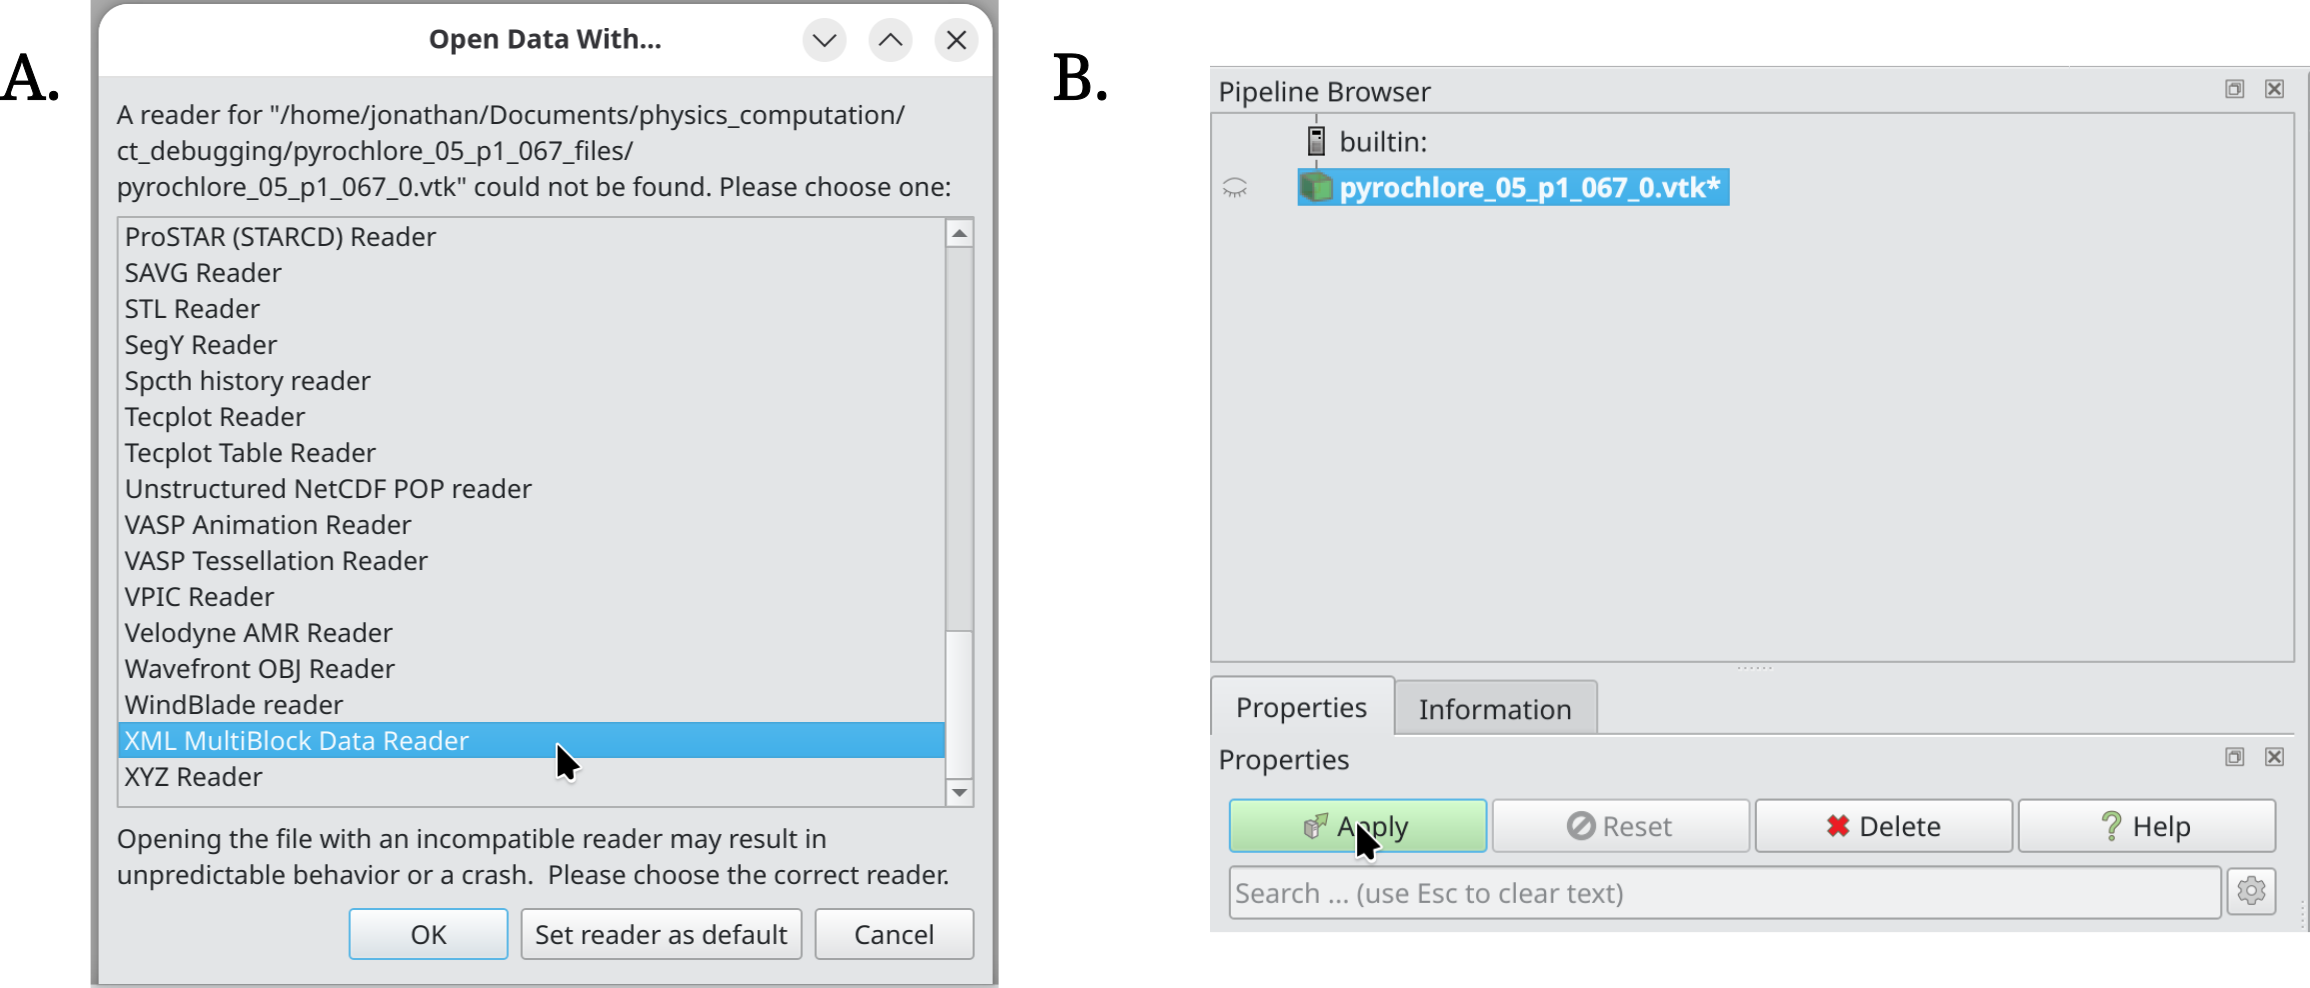
\includegraphics[width=.9\textwidth]{illustrations/file_loading_instructions}
\caption{Upon loading a .vtk file or a series of such files, the user selects
``\textsf{\textmd{XML Multiblock Data Reader}}'' from the resulting dialog
and then ``applies'' the resulting data to the current visualization workspace.}
\label{fig:load_files}
\end{figure}

\subsubsection{Split the data into pieces}
Different visualization procedures should be used for the network and gel
phases. These phases can be extracted using the \textsf{\textmd{Extract block}} 
tool in the upper toolbar. Use this tool twice to separately extract

Use this tool to separately extract \textsf{Block0} (the network), and 
\textsf{Block1} (the FEM mesh) by checking the appropriate box in the left-hand
tool panel and clicking \textsf{\textmd{Apply}}, as shown in Figure
\ref{fig:extract}.

\begin{figure}[h]
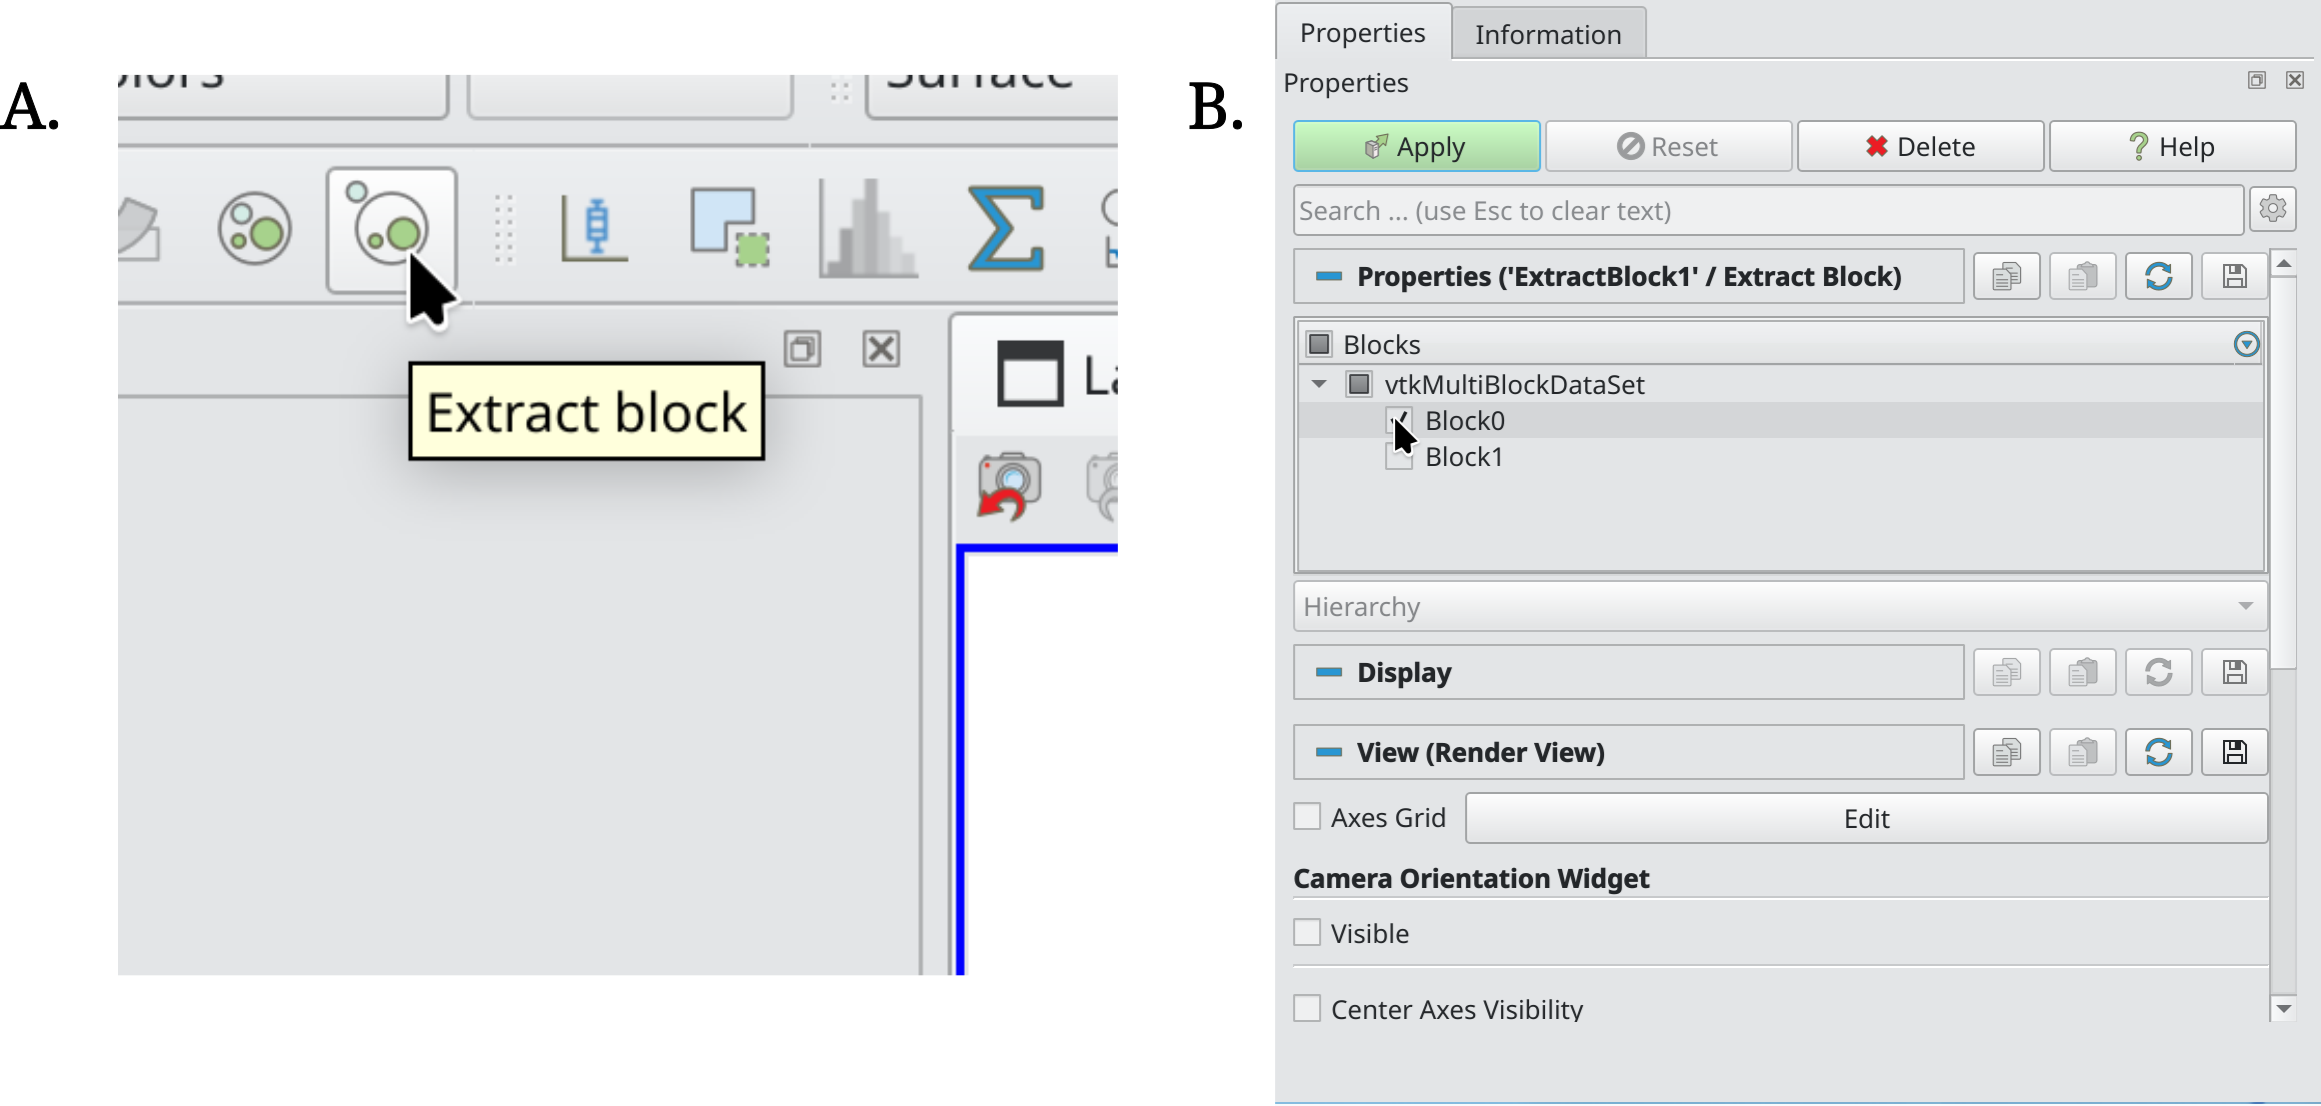
\includegraphics[width=.9\textwidth]{illustrations/extraction_illustration}
\caption{Use the extract tool to separate different components of the visualization, allowing distinct procedures to be performed on each component.}
\label{fig:extract}
\end{figure}

\subsubsection{Enhance the visualization of the network}
After splitting the visualization into separate blocks, right-click on the
first block and, from the resulting series of pop-up menus, select
\begin{center}
\textsf{\textmd{Add filter}} $\to$ \textsf{\textmd{Alphabetical}} $\to$
\textsf{\textmd{Tube}}, as shown in Figure ~\ref{fig:tube}.
\end{center}

\begin{figure}[H]
\begin{center}
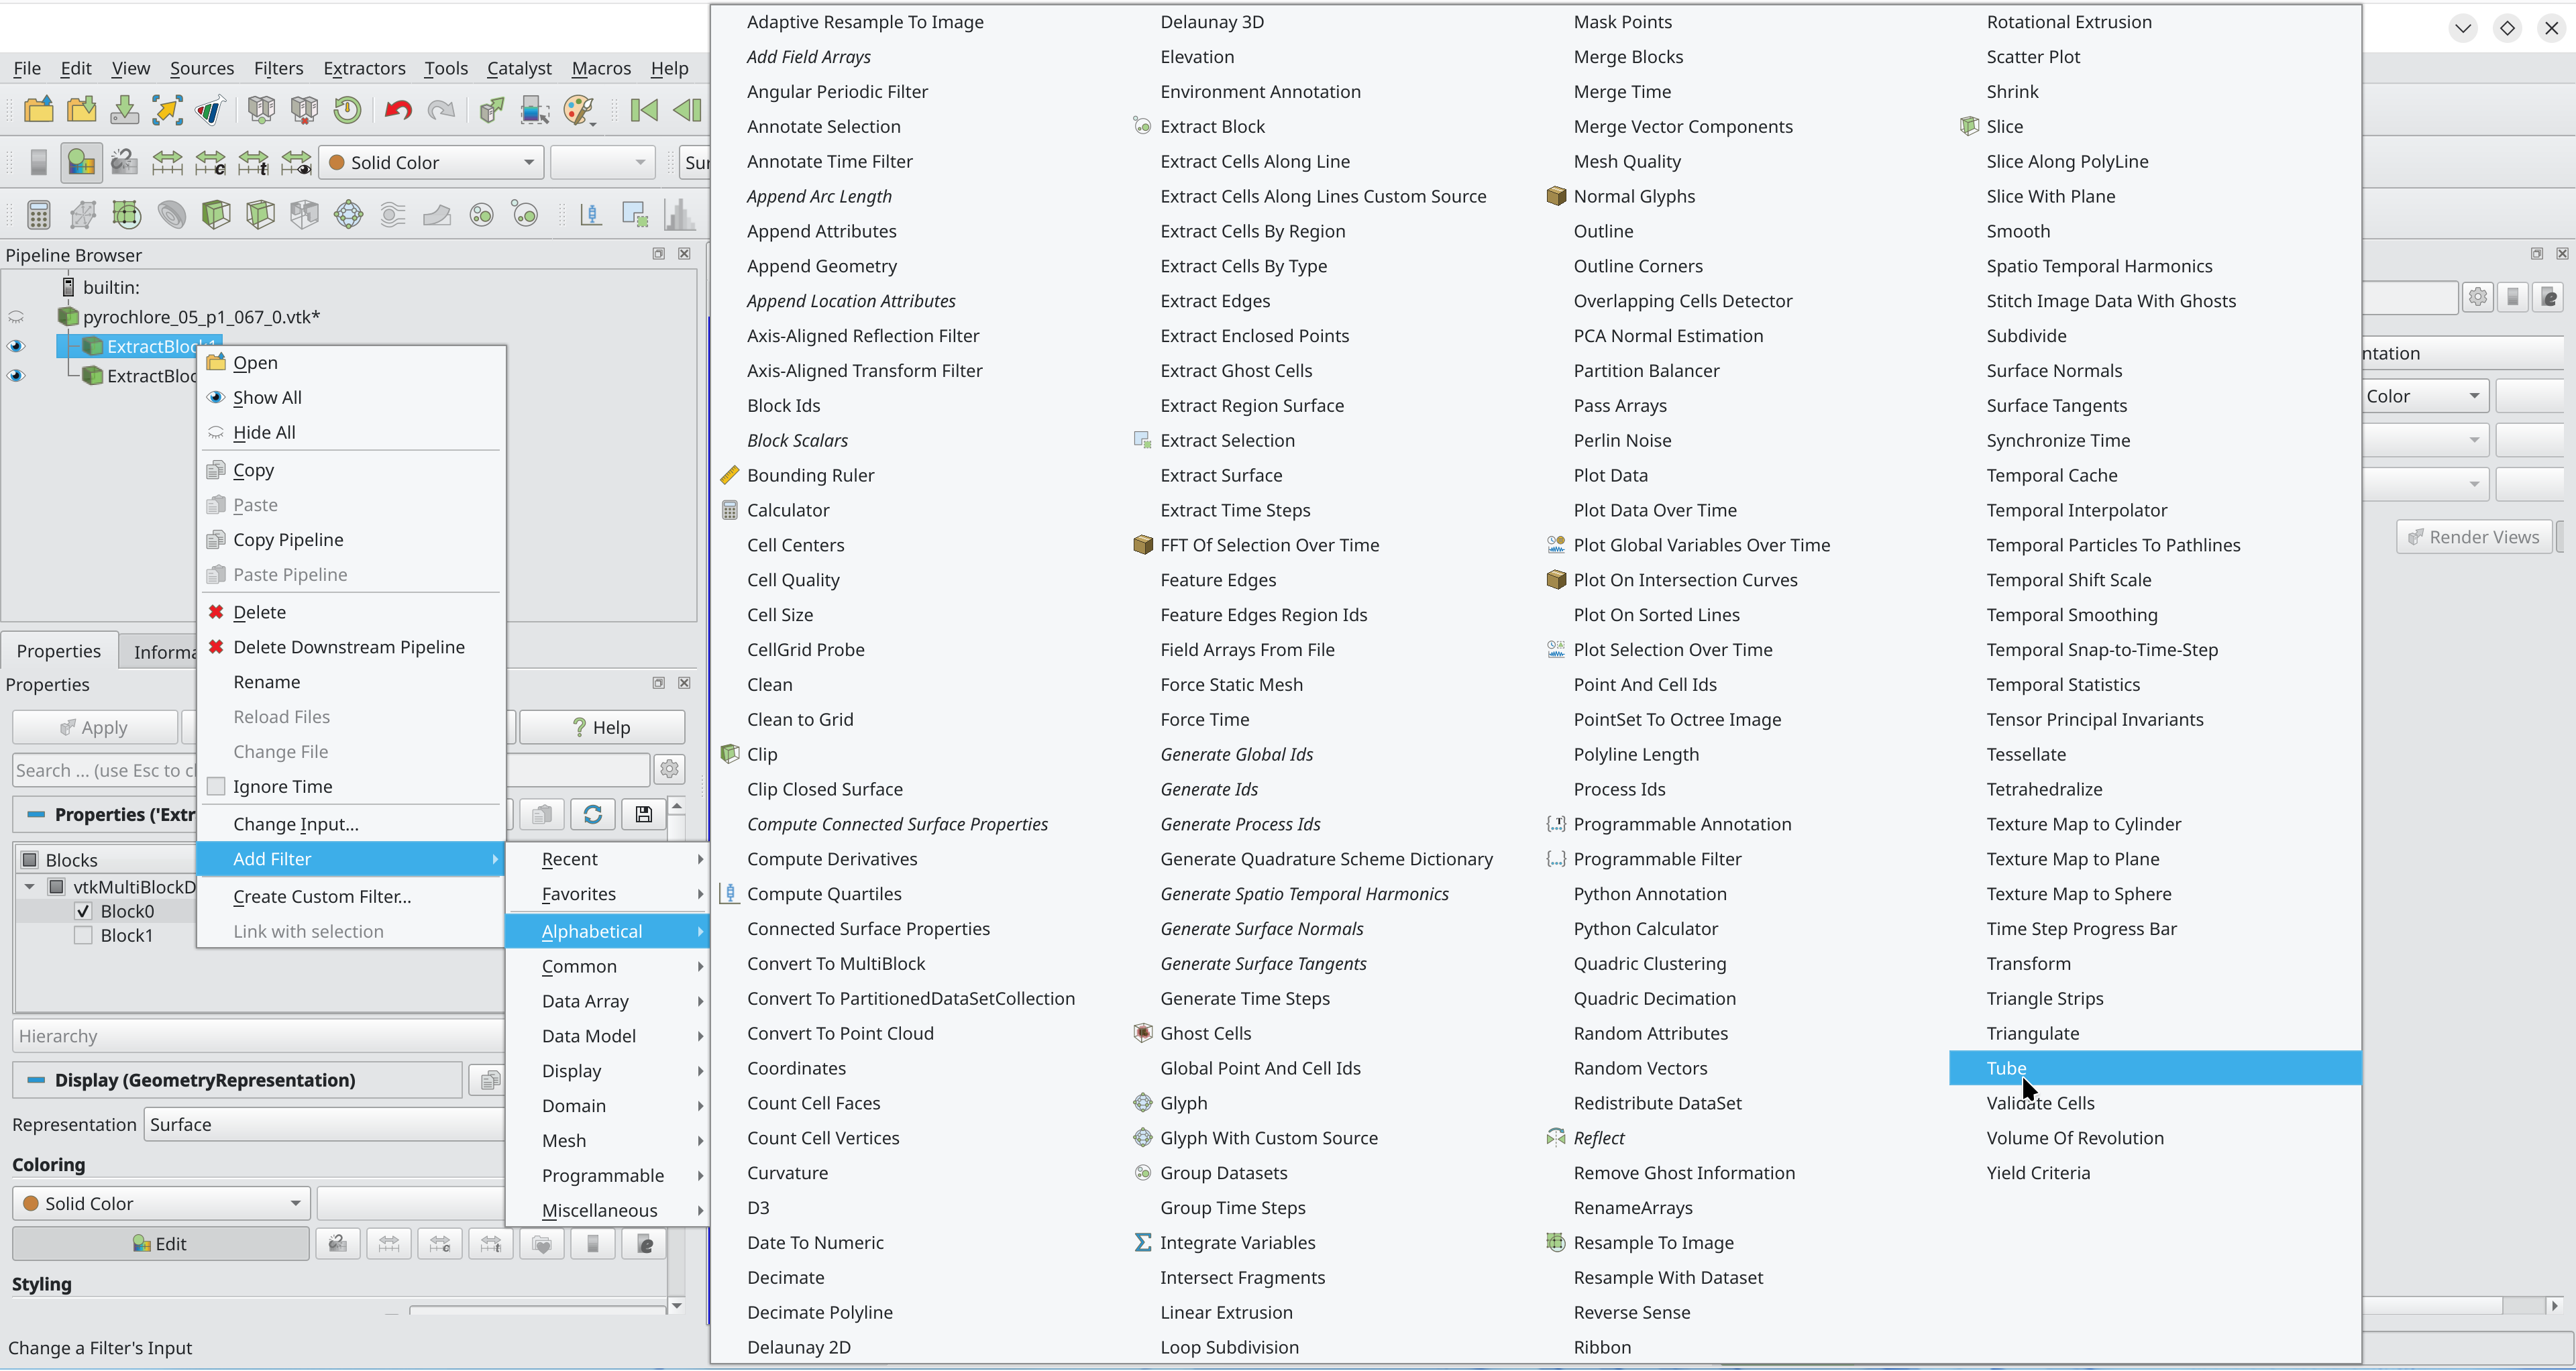
\includegraphics[width=\textwidth]{illustrations/apply_tube}
\end{center}
\caption{Apply the ``\textsf{\textmd{Tube}}'' filter to give some body to the
lines of the network.}
\label{fig:tube}
\end{figure}

\subsubsection{Fine-Tune the Appearance}
Once you have created the extraction blocks and added the tube visualization,
you can refine the appearance of the visualization. By clicking on one of
the visualization components in the upper left-hand 
\textsf{\textmd{Pipeline Browser}} pane, you can select options according
to context, such as the radius, number of sides, and color of tubes, or the
color and opacity used to visualize the finite element mesh.

\subsubsection{Step Through the Simulation}
If you are visualizing a multi-displacement simulation series, you will have
the option to use the forward and backward arrow buttons in the top tool bar
(see Figure ~\ref{fig:frame_toolbar}) to visualize the simulated experiment.
You can also play the simulation like a movie (although it will probably be a
rather short movie). An example sequence showing uniaxial compression and shear
is provided in Figure ~\ref{fig:example_simulation_viz}.

\begin{figure}
\begin{center}

\includegraphics[width=.7\textwidth]{illustrations/frame_toolbar}
\end{center}
\caption{Use the frame selection panel in the top tool bar to advance or
decrement the frame being displayed, or to play the series of visualizations.}
\label{fig:frame_toolbar}
\end{figure}

\begin{figure}
\begin{center}
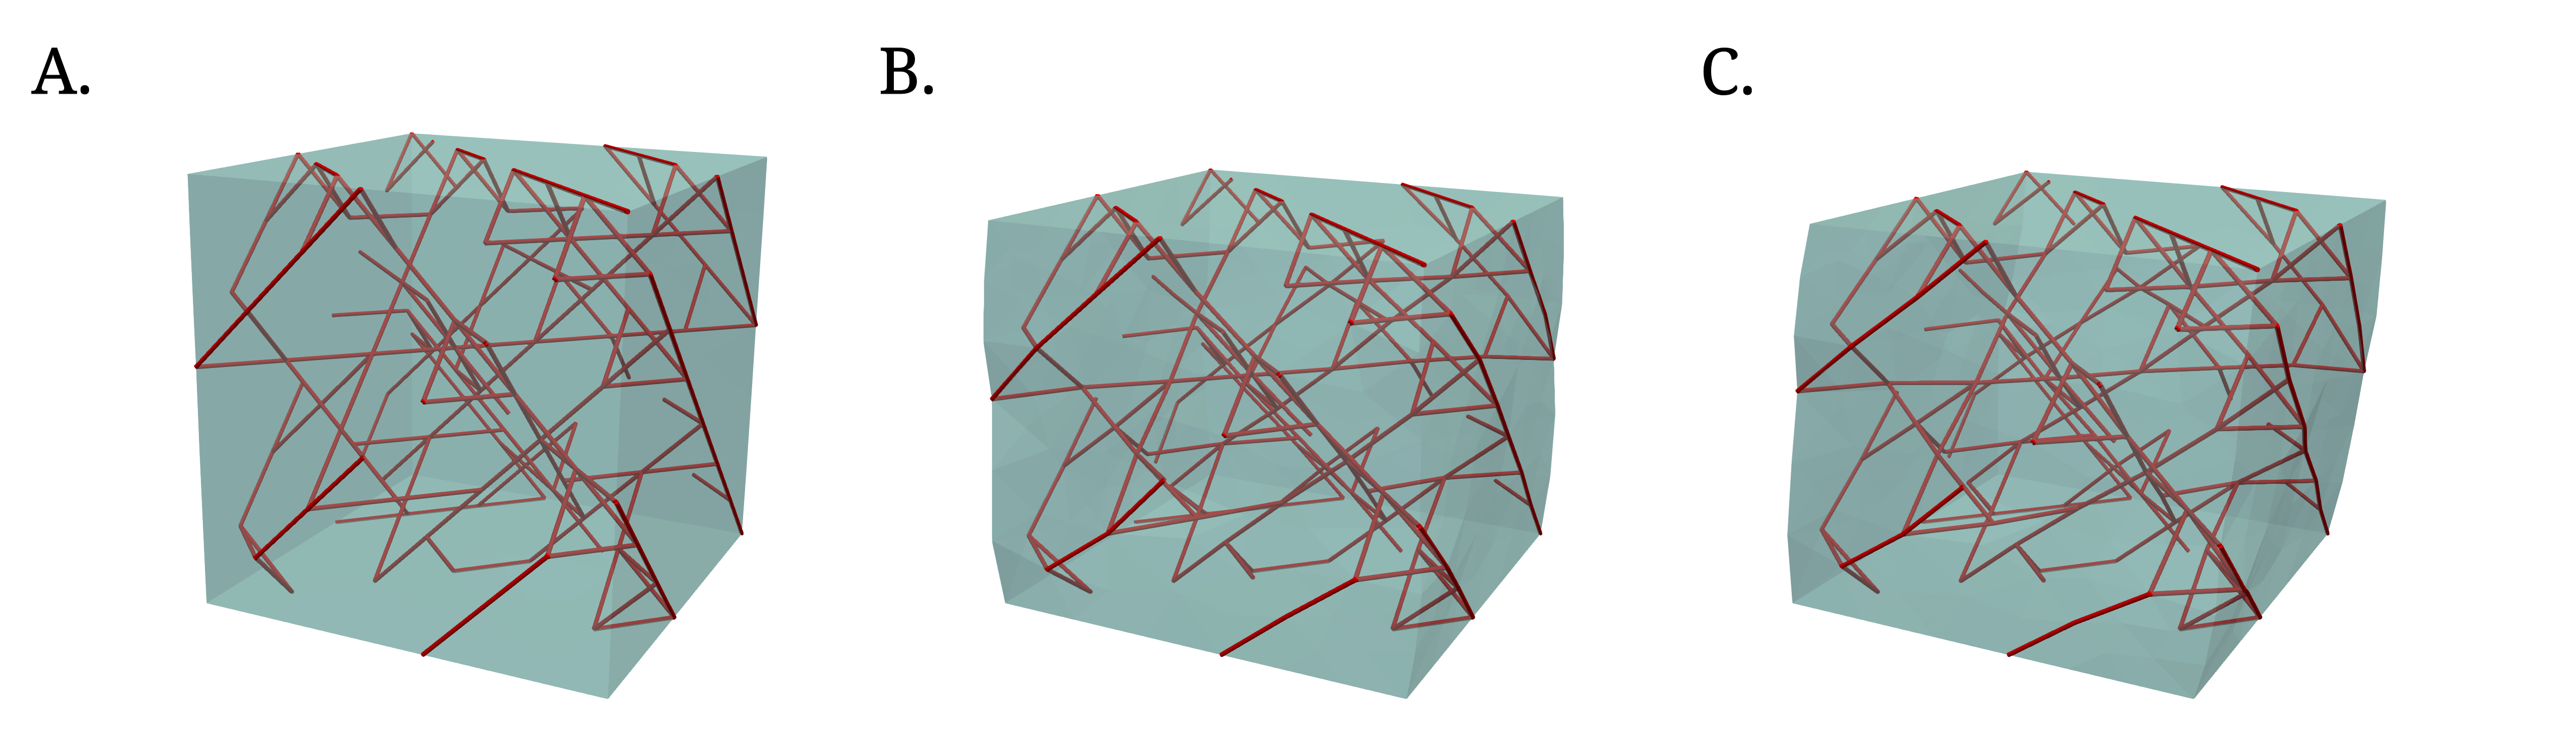
\includegraphics[width=\textwidth]{illustrations/pyrochlore_05_p1_067_compression_shear_sequence}
\end{center}
\caption{Here, we show a simulated experiment in which a tissue sample is
allowed to reach its swelling equilibrium (\textbf{A}), subjected to uniaxial
compression (\textbf{B}), and then sheard (\textbf{C}). The coordinate system
is oriented such that the $+\hat{z}$ axis points up, and the $+\hat{x}$ axis
points to the right and out of the page.}
\label{fig:example_simulation_viz}.
\end{figure}

\section{Auxiliary Utilities}

In setting up a parameter sweep, it is important to ensure your NMCs are
properly structured, and that you have chosen a physically sound set of
parameters for your physical model. For this purpose, two utilities that have
proven to be of use to the author have been included in the distribution:
\texttt{nmc\_stats}, which supplies statistics about the network edges, bending
triples, and tetrahedra, and \texttt{eq}, a program for anticipating the
equilibrium swelling volume of a gel, given the supplied constitutive model.
The use of both these programs is described here.

\subsection{\texttt{nmc\_stats}}

The program \texttt{nmc\_stats} expects one of two sets of arguments:
\begin{center}
\texttt{./nmc\_stats -n input\_file.nmc -o output\_name\_pattern}
\\or
\texttt{./nmc\_stats -d input\_file.dnmc -o output\_name\_pattern},
\end{center}
where ``\texttt{-n}'' is appropriate for .nmc files and ``\texttt{-d}'' is
appropriate for .dnmc files. This will result in four output files:

\begin{itemize}
\item \texttt{output\_name\_pattern\_summary.txt}
\item \texttt{output\_name\_pattern\_con\_hist.txt}
\item \texttt{output\_name\_pattern\_length\_hist.txt}
\item \texttt{output\_name\_pattern\_angle\_hist.txt}
\item \texttt{output\_name\_pattern\_tet\_vol\_hist.txt}
\end{itemize}

The summary file gives the numbers of edges, vertices, angles, and tetrahedra,
as well as the minimum, maximum, mean and standard devation for edge lengths,
vertex connectivities, equilibrium angles of bending triples, and tetrahedron
volumes. The accompanying histogram files give histogram data for each of these
quantities.

\subsection{\texttt{eq}}

This program takes as its arguments a job file appropriate for use with
\texttt{ngreleax} and an optional number of Newton's method steps for
computing the equilibrium swelling volume of the gel. In numerical experiments
performed while testing this code, convergence was generally rapid, with
a step limit of order $10$ sufficing. Assuming the directory containing
executables has been added to the environment variable \texttt{PATH}, one types:

\begin{center}
\texttt{eq job\_file\_name.json}
\end{center}
The resulting output will be the relative swelling volume of the gel.

\nocite{*}
\bibliographystyle{plain}
\bibliography{ctms_manual}{}

\appendix

\section{The Net3D File Format}

The Net3D file format is a simple extension of the XML standard, used to
generate lattice-based networks in the Composite Tissue Mechanics Suite. The 
geometrical structure of a network is broken into three units: points, rows,
and slices. The topology of the network is determined by listing neighbors
of points, which are specified by vectors from a given point to other points
to which it is connected. These relationships should only be specified in
one direction. By convention, Net3D files end with the extension
``\texttt{.n3d}''. In the following subsections, we describe each element of
a Net3D file.

\subsection{\texttt{net3d}}
The \texttt{net3d} element must always be the top-level element of a Net3D file.
This element contains as sub-elements all data needed to construct a
lattice-based network. The immediate child elements of the \texttt{net3d}
element are slices, which specify how points should be placed in a stack of
parallel planes, and how those points should be interconnected.

\subsection{\texttt{slice}}
The \texttt{slice} element contains a series of rows of points, all lying
in the same plane, with the plane normal in the $\hat{z}$ direction. The opening
tag of the \texttt{slice} element should specify the attribute \texttt{zoff}.
This is the offset, along the $+\hat{z}$ direction, from the current slice to
the next slice in the sequence. The one direct child element of the
\texttt{slice} element is the \texttt{row} element. After a set of slices is
loaded from a Net3D file, network construction will proceed by cycling through 
the specified sequence of slices, repeating as necessary until the desired
simulation volume is filled.

\subsection{\texttt{row}}
The \texttt{row} element describes a series of points with common $y$ and $z$
coordinates. The opening tag of the row element should specify the attributes
\texttt{x\_off} and \texttt{y\_off}. \texttt{x\_off} specifies the offset along
the $+\hat{x}$ direction from the minimum $x$ coordinate of the simulation box
to the first point in the row. \texttt{y\_off} specifies the offset along the
$+\hat{y}$ axis from the current row to the next row. In constructing a slice,
the library will repeat a sequence of rows to span the specified extent of the
simulation box along the $\hat{y}$ direction. The direct child of the
\texttt{row} element is the \texttt{point} element.

\subsection{\texttt{point}}
The \texttt{point} element specifies a single vertex within the network. The
Cartesian coordinates are not specified directly; instead, they are inferred
by adding up sets of offsets along the $x$, $y$, and $z$ directions as the
the network is built up through a series of points, rows, and slices. The
opening tag of the \texttt{point} field should specify the attribute
\texttt{to\_next}. This gives the displacement, along the $+\hat{x}$ direction,
from the current point to the next point within the current row. \texttt{point}
elements have as their children zero or more \texttt{neighbor} elements.

\subsection{\texttt{neighbor}}
The \texttt{neighbor} element is at the bottom of the Net3D file hierarchy.
Neighbors specify Cartesian offsets from points to neighboring points. The
components of these vectors are specified by the attributes \texttt{dx},
\texttt{dy}, and \texttt{dz}. As noted above, it is important that connections
between points only be  specified once: if the edge $(i, j)$ in the network is
specified, the edge  $(j, i)$ is implied, and should not be specified. Let
vertices $i$ and $j$ have positions $\vec{r}_i$ and $\vec{r}_j$, respectively,
and let \mbox{$\vec{d}_{ij} \equiv \vec{r}_j - \vec{r}_i$}. When choosing
whether to specify $\vec{d}_{ij}$ or $\vec{d}_{ji}$ explicitly, we have used
the convention that the greater of the two should be specified, as determined
by first comparing $z$ coordinates, then $y$ coordinates, and finally $x$
coordinates. The \texttt{neighbor} element has no children.

\subsection{A Simple Example}
To illustrate the concepts described above, we include below a Net3D file
describing the simple cubic lattice with nearest neighbor connections, included
with the default set of .n3d files in the Composite Tissue Mechanics Suite. This
network is not expected to be of much interest for research, but is presented
here as it offers the simplest comprehensive demonstration of the description
of a network.

\begin{figure}[!htb]
\framebox[\textwidth]{
\begin{minipage}[c]{\textwidth}
\texttt{
\\<?xml version="1.0" encoding="UTF-8"?>
\newline
\\<net3d>
\\\hspace*{4ex}<slice z\_off="1.000">
\\\hspace*{8ex}<row x\_off="0.000" y\_off="1.000">
\\\hspace*{12ex}<point to\_next = "1.000">
\\\hspace*{16ex}neighbor dx="1.000" dy="0.000" dz="0.000"/>
\\\hspace*{16ex}<neighbor dx="0.000" dy="1.000" dz="0.000"/>
\\\hspace*{16ex}<neighbor dx="0.000" dy="0.000" dz="1.000"/>
\\\hspace*{12ex}</point>
\\\hspace*{8ex}</row>
\\\hspace*{4ex}</slice>
\\</net3d>
}
\end{minipage}
}
\caption{This Net3D file generates a simple cubic lattice with nearest
neighbor bonds.}
\label{fig:sc_n3d_file}
\end{figure}

\section{libmatheval}
\label{sec:matheval}
The Composite Tissue Mechanics Suite uses the libmatheval library, a part of
the GNU project, to parse expressions representing gel free energies,
construct internal representations of energies, and automatically evaluate
necessary derivatives. To aid the user in entering expressions that will be
sucessfully parsed by libmatheval, we provide tables below of symbols used
by the libmatheval parser to represent mathematical constants
~\ref{tab:constants} and functions ~\ref{tab:functions}. Any user-defined
parameters must use names distinct from these names, and only the specified
functions below are currently supported.

Apart from named constants and functions, the library supports
altering priority of operations using parentheses, the unary negation operator,
indicated by ``$-$'', and the following binary operations: addition (``$+$''),
subtraction (``$-$''), multiplication (``$\ast$''), division (``$/$'') and
exponentiation (``$\wedge$''). Further information can be obtained from the
\href{https://www.gnu.org/software/libmatheval/}{project website}.

\begin{table}
\begin{center}
\caption{Recognized Mathematical Constants}
\label{tab:constants}
\vspace{1ex}
\begin{tabular}{l|r}
Quantity & Symbol \\
\hline
$e$ & \texttt{e}\\
$\log_2(e)$ & \texttt{log2e} \\
$\log_{10}(e)$ & \texttt{log10e} \\
$\ln(2)$ & \texttt{ln2} \\
$\ln(10)$ & \texttt{ln10}\\
$\pi$ & \texttt{pi}\\
$\pi / 2$ & \texttt{pi\_2}\\
$\pi / 4$ & \texttt{pi\_4}\\
$1 / \pi$ & \texttt{1\_pi}\\
$2 / \pi$ & \texttt{2\_pi}\\
$2 / \sqrt{\pi}$ & \texttt{2\_sqrtpi}\\
$\sqrt{2}$ & \texttt{sqrt2}\\
$\sqrt{1 / 2}$ & \texttt{sqrt1\_2}
\end{tabular}
\end{center}
\end{table}

\begin{table}
\begin{center}
\caption{Recognized Functions}
\label{tab:functions}
\vspace{1ex}
\begin{tabular}{l|r}
Function & Symbol \\
\hline
exponential & \texttt{exp}\\
natural logarithm & \texttt{log}\\
square root & \texttt{sqrt}\\
sine & \texttt{sin}\\
cosine & \texttt{cos}\\
tangent & \texttt{tan}\\
cotangent & \texttt{cot}\\
secant & \texttt{sec}\\
cosecant & \texttt{csc}\\
inverse sine & \texttt{asin}\\
inverse cosine & \texttt{acos}\\
inverse tangent & \texttt{atan}\\
inverse cotangent & \texttt{acot}\\
inverse secant & \texttt{asec}\\
inverse cosecant & \texttt{acsc}\\
hyperbolic sine & \texttt{sinh}\\
hyperbolic cosine & \texttt{cosh}\\
hyperbolic tangent & \texttt{tanh}\\
hyperbolic cotangent & \texttt{coth}\\
hyperbolic secant & \texttt{sech}\\
hyperbolic cosecant & \texttt{csch}\\
hyperbolic inverse sine & \texttt{asinh}\\
hyperbolic inverse cosine & \texttt{acosh}\\
hyperbolic inverse tangent & \texttt{atanh}\\
hyperbolic inverse secant & \texttt{asech}\\
hyperbolic inverse cosecant & \texttt{acsch}\\
absolute value & \texttt{abs}\\
Heaviside step function ($x\left(0\right) \equiv 0$) & \texttt{step}\\
Dirac delta, $\delta(x) \equiv \inf$ & \texttt{delta}\\
Dirac delta, $\delta(x) \equiv \text{not-a-number}$ & \texttt{nandelta}\\
Error function & \texttt{erf}
\end{tabular}
\end{center}
\end{table}

\end{document}
